% !TEX encoding = UTF-8 Unicode
% !TEX TS-program = pdflatex
% !TEX root = ../Tesi.tex



%************************************************
\myChapter{Elaborazione dei risultati}
%************************************************
\label{cap:output}
In questo capitolo verrà posta attenzione sull'estrazione di risultati utili dalle analisi numeriche svolte:
\begin{itemize}
\item Forze e coppie
\item Induttanze
\item Capacità
\end{itemize}
\section{Forze e coppie}
Il calcolo di forze e coppie elettromagnetiche è di primaria importanza nell'ambito dell'analisi di dispositivi elettromeccanici. 

Tuttavia, come si vedrà in questo capitolo, è tutt'altro che agevole laddove non si debbano calcolare forze su cariche note, siano esse ferme o in movimento. 
Un esempio è il magnete permanente: come si è visto nel capitolo \ref{cap:maxwell}, l'orientamento delle orbite elettroniche all'interno dei domini è un fenomeno stocastico rappresentato tramite un modello macroscopicamente equivalente. Tale modello non è adatto al calcolo diretto delle forze agenti sulle cariche \textit{reali} in movimento all'interno del mezzo. Si rende pertanto necessario l'utilizzo di specifiche tecniche per il calcolo delle forze scambiate fra magneti permanenti.

Iniziamo quindi introducendo le forze agenti in un volume in cui vi sia una densità di carica $\rho$ in moto con velocità $\T{v}$:

\begin{align}
\label{eq:5coulombf}
&\text{Forza di \textit{Coulomb}} &\T{f_c}=\rho \T{e}  \\
\label{eq:5lorentzf}
&\text{Forza di \textit{Lorentz}}&\T{f_l}=\rho \T{v}\times \T{b} .
\end{align}

Si ottiene quindi la forza totale esercitata dai due campi:
\begin{equation}
\label{eq:5ftot1}
\T{f}=\rho \left(\T{e}+\T{v}\times \T{b}\right).
\end{equation}

Nel caso in cui vi siano soltanto cariche in quiete e cariche in movimento modellabili come correnti stazionarie la forza totale può essere espressa come:
\begin{equation}
\label{eq:5ftot2}
\T{f}=\rho\T{e} +\T{j}\times \T{b}.
\end{equation}

Laddove le forze non possano essere espresse tramite le espressioni di Lorentz e Coulomb, vengono adottati metodi di origine diversa, che si differenziano per precisione, difficoltà di implementazione, praticità di utilizzo.
\subsection{Metodo delle cariche magnetiche equivalenti}
 Questo metodo consiste nella modellazione della magnetizzazione residua $\T{m_r}$ tramite una distribuzione di cariche virtuali nel volume e sulla superficie del magnete:
\begin{align}
\label{eq:5cariche_eq1a}
&\rho =-\dive \left(\T{m_r}\right) \qquad  &\text{in $V$,}\\
\label{eq:5cariche_eq1b}
&\rho_s =\T{m_r}\cdot \T{n} \qquad &\text{in $\de V$.}
\end{align}
Sotto l'azione di un campo magnetico esterno si ottiene quindi una forza \citep{furlani_permanent_2001}:
\begin{equation}
\label{eq:5sourcef}
\T{F} = \int_V \rho\T{b} dv+\int_{\de V} \rho_s \T{b} ds. 
\end{equation}
Si può osservare come nel caso di magnetizzazione costante nei diversi domini le forze siano superficiali.
Nel caso in cui vi siano domini con diverse magnetizzazioni adiacenti, considerando l'orientazione delle rispettive normali con riferimento alla Figura \ref{fig:5.1}, si ha per i termini di superficie:
\begin{align}
\label{eq:5sourcef2}
\T{f_{s1}}&=\left(\T{n_1}\cdot\T{m_{r1}}\right)\bar{\T{b}}\nonumber\\
\T{f_{s2}}&=\left(\T{n_2}\cdot\T{m_{r2}}\right)\bar{\T{b}}\nonumber\\
\T{f_{s}}&=\langle\T{n}\cdot\T{m_{r}}\rangle\bar{\T{b}},
\end{align}
dove $\bar{\T{b}}$ è la media dell'induzione magnetica a cavallo dell'interfaccia ($\bar{\T{b}}=\left(\T{b_1}+\T{b_2}\right)/2$).
\begin{SCfigure}
\caption{Domini per il calcolo di forze superficiali tramite cariche e correnti equivalenti}
\label{fig:5.1}
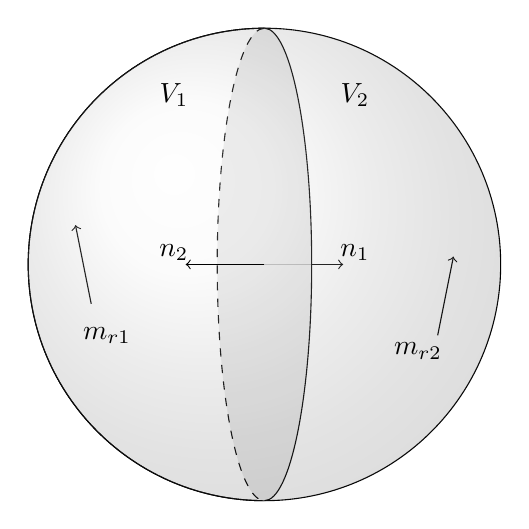
\begin{tikzpicture}
\draw[black] (0,0) circle (3);
\draw[black] (0,3) arc (90:270:3);
\draw[->] (0,0) -- (1,0);
\fill[black!10!white, opacity = .8] (0,0) ellipse (.6 and 3);
\draw[dashed] (0,3) arc (90:270:.6 and 3);
\draw (0,3) arc (450:270:.6 and 3);
\draw[->] (2.2,-0.9) -- (2.4,.1);
\draw[->] (-2.2,-.5) -- (-2.4,0.5);
\shade[ball color=black!10!white,opacity=0.20] (0,0) circle (3);

\draw[->] (0,0) -- (-1,0);
\draw (-2,-.9) node {$\T{m_{r1}}$}; %label
\draw (1.95,-1.1) node {$\T{m_{r2}}$}; %label
\draw (1.15,0.15) node {$\T{n_1}$}; %label
\draw (-1.15,0.15) node {$\T{n_2}$}; %label
\draw (1.15,2.15) node {$V_2$}; %label
\draw (-1.15,2.15) node {$V_1$}; %label
\end{tikzpicture}
\end{SCfigure}
\subsection{Metodo delle correnti magnetiche equivalenti} Come nel metodo precedente si cerca un'espressione della magnetizzazione residua; in questo caso viene adottato un modello a correnti:
\begin{align}
\label{eq:5correnti_eq1a}
&\T{j} =\rot\left(\T{m_r}\right) \qquad  &\text{in $V$,}\\
\label{eq:5correnti_eq1b}
&\T{j_s} =\T{m_r}\times \T{n} \qquad &\text{in $\de V$.}
\end{align}
Riscriviamo la forza di Lorentz:
\begin{equation}
\label{eq:5currentf}
\T{F} = \int_V \T{j}\times\T{b} dv+\int_{\de V} \T{j_s} \times \T{b} ds. 
\end{equation}
Anche in questo caso otteniamo i termini di superficie nel caso di due domini adiacenti:
\begin{align}
\label{eq:5currentf2}
\T{f_{s}}&=\langle\T{m_{r}}\times\T{n}\rangle\times\bar{\T{b}}.
\end{align}
Si sottolinea qui che i due metodi appena presentati forniscono solo una rappresentazione globale equivalente ai fini del calcolo del campo magnetico al di fuori del dominio dei magneti permanenti; permettono pertanto soltanto il calcolo delle forze risultanti (e delle relative coppie) e non delle forze distribuite (locali) \citep{de_medeiros_about_1999}.
\subsection{Tensore di Maxwell} Questo strumento molto versatile permette di calcolare forze di origine elettrica e magnetica in un contesto assolutamente generale, indipendente dal regime utilizzato e dalla natura delle forze che originano i campi.

Si inizi esplicitando i termini $\rho$ e $\T{j}$ dall'equazione \eqref{eq:5ftot2} in funzione del campo elettrico $\T{e}$ e dell'induzione magnetica $\T{b}$:
\begin{align}
\label{eq:5maxf1}
\T{f}&=\dive\left(\T{d}\right) \T{e} +\left[\rot\left(\T{h}\right)-\de_t \T{d}\right]\times \T{b}\nonumber\\
&=\varepsilon\dive\left(\T{e}\right) \T{e} +\left[\mu^{-1}\rot\left(\T{b}\right)-\varepsilon\de_t \T{e}\right]\times \T{b}.
\end{align}

Si utilizzi la relazione:
\begin{equation}
\label{eq:5vectid}
\de_t\left(\T{e}\times\T{b}\right) = \de_t \T{e}\times \T{b} + \T{e}\times\de_t\T{b}
\end{equation}
per riscrivere l'ultimo termine dell'equazione \eqref{eq:5maxf1}:
\begin{align}
\label{eq:5maxf2}
\T{f}=\varepsilon\dive\left(\T{e}\right) \T{e} &+\mu^{-1}\rot\left(\T{b}\right)\times \T{b}+\nonumber\\
&-\varepsilon \left[\de_t\left(\T{e}\times\T{b}\right)-\T{e}\times\de_t\T{b}\right]
\end{align}
e, per la legge di Faraday,
\begin{align}
\label{eq:5maxf3}
\T{f}=\varepsilon\dive\left(\T{e}\right) \T{e} &+\mu^{-1}\rot\left(\T{b}\right)\times \T{b}+\nonumber\\
&-\varepsilon \left[\de_t\left(\T{e}\times\T{b}\right)+\T{e}\times\rot\left(\T{e}\right)\right].
\end{align}
Per simmetria, si aggiunga il termine (identicamente nullo) $\mu^{-1} \dive\left(\T{b}\right)\T{b}$:
\begin{align}
\label{eq:5maxf4}
\T{f}=\varepsilon\dive\left(\T{e}\right) \T{e} +\mu^{-1} \dive\left(\T{b}\right)\T{b}+\nonumber\\
-\mu^{-1}\T{b}\times\rot\left(\T{b}\right) -\varepsilon\T{e}\times\rot\left(\T{e}\right)+\nonumber\\
-\varepsilon\de_t\left(\T{e}\times\T{b}\right).
\end{align}
Si utilizzi ora l'identità vettoriale
\begin{equation}
\label{eq:5vectid2}
\grad\left(\T{v}\cdot\T{v}\right) = 2 \T{v}\times\rot\left(\T{v}\right)+2\grad\left(\T{v}\right)\T{v}
\end{equation}
così da ottenere
\begin{align}
\label{eq:5maxf5}
\T{f}=\varepsilon \left[ \dive \left( \T{e} \right) \T{e} + \grad \left( \T{e} \right) \T{e} \right] +\nonumber\\
+\mu^{-1} \left[\dive\left(\T{b}\right)\T{b}+\grad\left(\T{b}\right)\T{b}\right] +\nonumber\\
-\frac{1}{2} \grad\left[\varepsilon\left(\T{e}\cdot\T{e}\right)+
\mu^{-1}\left(\T{b}\cdot\T{b}\right) \right] +\nonumber\\
-\varepsilon\de_t\left(\T{e}\times\T{b}\right).
\end{align}
In questo modo la forza per unità di volume può essere espressa in funzione del \textit{vettore di Poynting} $\T{s}$ e del \textit{tensore di Maxwell} $\TT{T}$ \citep{griffiths_introduction_2013}:
\begin{equation}
\label{eq:5poyntandmax}
\left\{
\begin{aligned}
\T{s} &= \mu^{-1} \T{e}\times\T{b}\\
\TT{T} &= \varepsilon\left[\T{e}\otimes\T{e} -\frac{1}{2}\left(\T{e}\cdot\T{e}\right)\TT{I}\right] +
\mu^{-1}\left[\T{b}\otimes\T{b} -\frac{1}{2}\left(\T{b}\cdot\T{b}\right)\TT{I}\right]
\end{aligned}
\right.
\end{equation}

\begin{equation}
\label{eq:5poyntandmax2}
\T{f} = \dive\left(\TT{T}\right) -\varepsilon\mu^{-1} \de_t\T{s},
\end{equation}

dove $\TT{I}$ è il tensore identità di secondo ordine. 

Nell'approccio ai regimi ridotti si elide il contributo dovuto al tensore di Poynting. In questo modo la forza elettromagnetica dipende solamente dal tensore di Maxwell.

Applicando ora il teorema di Gauss all'equazione \eqref{eq:5poyntandmax2} si ottiene un'espressione diretta della forza elettromagnetica totale in un volume $V$ tramite il calcolo del flusso del tensore di Maxwell:

\begin{equation}
\label{eq:5maxf6}
\int_V\T{f} = \int_V\dive\left(\TT{T}\right)dv = \int_{\de V}\TT{T}\cdot \T{n}ds.
\end{equation}

Questo importante risultato permette di ottenere forze (e coppie) totali agenti su un corpo scegliendo un'opportuna superficie che circondi il corpo. \'E importante sottolineare come il risultato numerico non sia indipendente dalla scelta della superficie; in particolare si osserva che se la superficie coincide (o è sufficientemente vicina) alla superficie fisica di un corpo non si ottengono risultati attendibili. Tale comportamento è particolarmente evidente nelle analisi 3D. \'E opportuno scegliere la superficie dove la distribuzione di forza (attesa) è più regolare possibile. 
Vengono qui elencati accorgimenti e limiti del metodo, ottenuti con prove numeriche.
\begin{enumerate}
\item La superficie \textit{non può} intersecare il confine tra due domini con proprietà elettromagnetiche diverse. Come visto nei capitoli precedenti, la condizione di interfaccia porta discontinuità nei campi.
\item  La superficie deve attraversare solamente materiali diamagnetici o ferromagnetici (tipicamente si sceglie l'aria che circonda i corpi).
\item La superficie deve essere sufficientemente lontana dalle sorgenti di campo.
\item Le superfici possono avere spigoli vivi, ma quanto più le superfici sono regolari tanto più il calcolo sarà accurato. Forme sferiche o calotte emisferiche portano in genere a buoni risultati.
\item Si può abbinare il questo metodo con la tecnica delle trasformazioni al contorno (vedi sezione \ref{sec:dominiaperti}): in questo caso, se si sceglie come volume racchiuso dalla superficie di Maxwell l'intero volume di calcolo, compresa la regione della \textit{shell boundary region}, il flusso del tensore all'infinito (la superficie esterna) è intrinsecamente nullo; le forze saranno così ottenute unicamente dal flusso che attraversa la superficie di interfaccia tra le due regioni (indicata in rosso in Figura \ref{fig:5.2}).
\end{enumerate}

\begin{figure}
\centering
\caption{Suddivisione delle regioni per un utilizzo abbinato del tensore di Maxwell e di una trasformazione al contorno}
\label{fig:5.2}
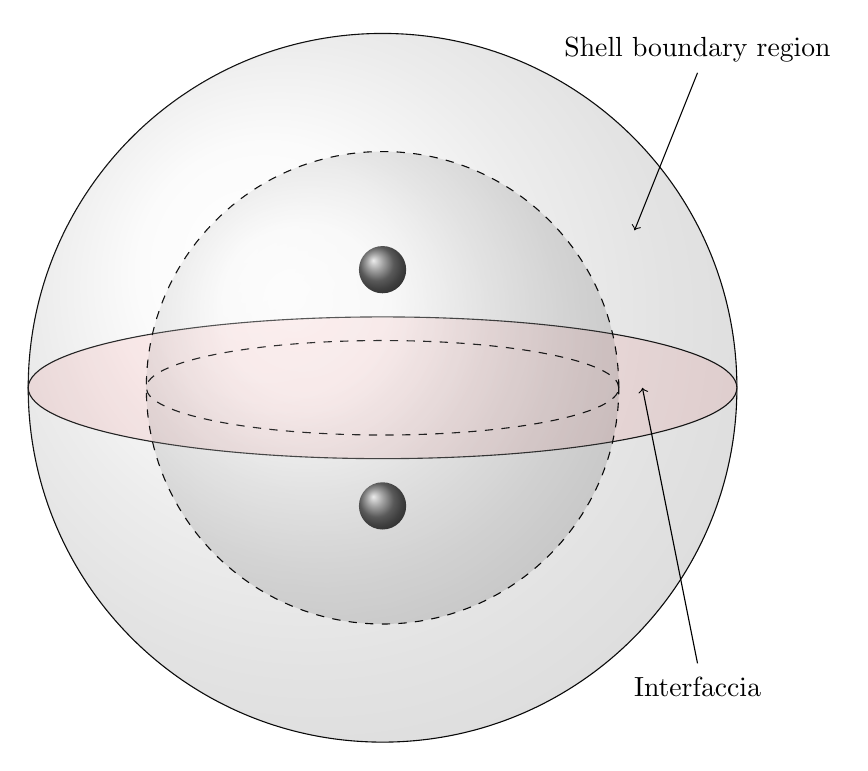
\begin{tikzpicture}
\draw[black] (0,0) circle (4.5);
\fill[red!10!white, opacity = .8] (0,0) ellipse (4.5 and .9);
\draw[black] (0,0) ellipse (4.5 and .9);
\shade[ball color=black!10!white,opacity=0.20] (0,0) circle (4.5);
\draw[black,dashed] (0,0) circle (3);
\draw[black,dashed] (0,0) ellipse (3 and .6);
\shade[ball color=black!10!white,opacity=0.20] (0,0) circle (3);
\shade[ball color=black!50!white,opacity=1] (0,1.5) circle (.3);
\shade[ball color=black!50!white,opacity=1] (0,-1.5) circle (.3);
\draw[->] (4,4) -- (3.2,2);
\draw (4,4.3) node {Shell boundary region}; %label
\draw[->] (4,-3.5) -- (3.3,0);
\draw (4.,-3.8) node {Interfaccia}; %label
\end{tikzpicture}
\end{figure}

\subsection{Principio dei Lavori Virtuali (PLV)}
Sotto questo nome rientrano i metodi che ottengono la forza a partire dall'energia del campo elettromagnetico. Tali metodi competono per generalità e applicabilità con il tensore di Maxwell.

Ci limiteremo al calcolo delle forze dovute al campo magnetico in quanto, come per i metodi precedenti, il grosso vantaggio è insito nel calcolo di forze dovute a magnetizzazioni permanenti.

Le forze di origine elettromagnetica sono ottenute grazie alla derivata dell'energia magnetica rispetto ad uno spostamento arbitrario.

Per questo il PLV può essere sfruttato in  due modi:
\begin{itemize}
\item Per ottenere forze e coppie globali esprimendo la variazione di energia magnetica rispetto al movimento (o alla rotazione) di un corpo secondo un grado di libertà rigido;
\item Per ottenere la distribuzione locale di forze magnetiche esprimendo la variazione di energia magnetica rispetto al movimento di ogni singolo grado di libertà degli elementi. 
\end{itemize}

Per le analisi successive è stato implementato unicamente il primo dei due metodi perché di più immediata realizzazione.

L'energia magnetica per unità di volume è esprimibile come:
\begin{equation}
w = \int \T{h}\cdot d\T{b}. 
\label{eq:5en1}
\end{equation}

Utilizzando il legame costitutivo \eqref{eq:2costmag} si ottiene:
\begin{equation}
w = \int \mu^{-1}\left(\T{b}-\T{b_r}\right) \cdot d\T{b}. 
\label{eq:5en2}
\end{equation}

In base alla scelta degli estremi di integrazione si ottengono varie espressioni dell'energia che, vista la linearità dell'espressione rispetto a $\T{b}$, differiscono per una costante \citep{henrotte_computation_2004}:
\begin{align}
\label{eq:5en3}
w &= \mu^{-1}\frac{\T{b}\cdot\T{b}}{2}\\
\label{eq:5en4}
w &= \mu^{-1}\left(\frac{\T{b}\cdot\T{b}}{2}-\T{b}\cdot\T{b_r}\right)\\
\label{eq:5en5}
w &= \mu^{-1}\frac{\left(\T{b}-\T{b_r}\right)\cdot\left(\T{b}-\T{b_r}\right)}{2}
\end{align}

Allo stesso modo l'energia complementare, per definizione
\begin{equation}
w' = \int \T{b}\cdot d\T{h} = \int \left(\mu\T{h}+\T{b_r}\right) \cdot d\T{b}
\label{eq:5enc1}
\end{equation}
assume (utilizzando il medesimo legame costitutivo) le diverse forme:
\begin{align}
\label{eq:5enc3}
w' &= \mu\frac{\T{h}\cdot\T{h}}{2}\\
\label{eq:5enc4}
w' &= \mu\frac{\T{h}\cdot\T{h}}{2}+\T{h}\cdot\T{b_r}\\
\label{eq:5enc5}
w' &= \mu\frac{\left(\T{h}+\T{m}\right)\cdot\left(\T{h}+\T{m}\right)}{2}
\end{align}
Poiché forze e coppie sono ottenute mediante variazioni di queste quantità, nel caso di legame costitutivo lineare tutte le espressioni sopra elencate sono equivalenti.\\

La forza meccanica di origine magnetica può essere calcolata integrando tali espressioni in tutto il dominio di analisi e calcolando la derivata (ad esempio tramite schemi alle differenze finite) rispetto allo spostamento dei nodi appartenenti al corpo analizzato :
\begin{align}
\label{eq:5fplv1_a}
F &= -\frac{\de\int_V w dv}{\de s} = -\de_s W\\
\label{eq:5fplv1_b}
F &= \frac{\de\int_V w' dv}{\de s} = \de_s W'\\
\label{eq:5fplv1_c}
C &= -\frac{\de\int_V w dv}{\de \theta} = -\de_{\theta} W\\
\label{eq:5fplv1_d}
C &= \frac{\de\int_V w' dv}{\de \theta} = \de_{\theta} W'\\
\end{align}

\'E evidente che nel caso di analisi in domini aperti è essenziale una corretta simulazione del decadimento dei campi nelle regioni lontane; quindi la presenza di una tecnica di modellazione come la SST presentata nel Capitolo \ref{cap:boundary} è essenziale. In questo caso è utile ricordare che nell'integrazione dell'energia nel volume esterno deve essere utilizzato anche lo jacobiano per ottenere un integrale il cui dominio è quello originario (aperto) e non quello trasformato (chiuso).

\subsection{Test-case: due fili in 2D (seconda parte)}

Si illustra qui il risultato ottenuto confrontando due dei metodi di calcolo precedentemente descritti per il caso test illustrato in Sezione \ref{subsec:2fili}:
il metodo della superficie di Maxwell e il metodo basato sul PLV.


Si è scelta come superficie di Maxwell una circonferenza attorno ai due fili di raggio variabile (Figura \ref{fig:2filimax}).
\begin{figure}[htb]
\centering
\caption{Dominio dei due fili e delle superfici di Maxwell che li circondano}
\label{fig:2filimax}

\includegraphics[width = .8\textwidth]{2filimax}
\end{figure}

In Tabella \ref{tab:fili2d2} sono mostrate le forze in direzione $x$ e $y$ per i due fili confrontando i metodi di Maxwell e del PLV con il valore teorico dato dalla formula di Lorentz. In tabella si fa riferimento al filo a nord con il pedice "N" e al filo a sud con il pedice "S".

\begin{table}[htb]
\caption{Confronto tra i valori di forza ottenuti tramite superficie di Maxwell e PLV}
\label{tab:fili2d2}
\centering
\begin{tabular}{lcccc}
\toprule
Metodo & $F_{xN}$ (N) & $F_{yN}$ (N) & $F_{xS}$  (N) & $F_{yS}$ (N)\\
\midrule
Lorentz & 0 & -5849.45 & 0 & 5849.45 \\
Maxwell & 2.43 & -5850.10 & 3.43 & 5850.40\\
PLV & 2.94& -5849.19 & 0.18 & 5850.57\\
\bottomrule
\end{tabular}
\end{table}

I risultati evidenziano che in due dimensioni e implementando una trasformazione al contorno i metodi sono estremamente precisi. In tre dimensioni e con l'aggiunta di magneti permanenti l'accuratezza del calcolo ottenuto peggiora notevolmente.

\subsection{Test-case: due magneti sferici in 3D}

Si illustra qui il risultato ottenuto confrontando tutti i metodi fin qui descritti per ottenere le forze scambiate tra due magneti di forma sferica con magnetizzazione costante, opposta e parallela alla retta che congiunge i centri delle due sfere. I dati geometrici utilizzati sono elencati in Tabella \ref{tab:2sfere} 

\begin{figure}[htb]
\centering
\caption{Porzioni della mesh racchiuse dalle superfici di Maxwell; la magnetizzazione  è costante (in direzione $x$), uguale ed opposta per le due sfere}
\label{fig:2sfere}

\includegraphics[width = .4\textwidth]{2sfere_a}
\quad 
\includegraphics[width = .4\textwidth]{2sfere_b}
\end{figure}

\begin{table}[htb]
\caption{Dati geometrici utilizzati per il caso test}
\label{tab:2sfere}
\centering
\begin{tabular}{lc}
\toprule
Raggio sfere & \begin{tabular}{cc}$r$ & 0.25 m\end{tabular}\\
Distanza tra i centri delle sfere & \begin{tabular}{cc}$d$ & 1.5 m\end{tabular}\\
Campo magnetico residuo & \begin{tabular}{cc}$\T{b_r}$ & 1.36 T\end{tabular}\\
Superficie di Maxwell (Prisma) & $5m\times 10m\times 10m$\\
\bottomrule
\end{tabular}
\end{table}

In Tabella \ref{tab:2sfere2} sono mostrate le forze nelle tre direzioni. Si fa riferimento alla sfera sinistra con il pedice "S" e quella destra con il pedice "D".\\

\begin{table}[htb]
\caption{Confronto tra i valori di forza ottenuti tramite superficie di Maxwell e PLV}
\label{tab:2sfere2}
\centering
\footnotesize
\begin{tabular}{lcccccc}
\toprule
Metodo & $F_{xS}$ (N) & $F_{yS}$ (N) & $F_{zS}$  (N) & $F_{xD}$ (N) & $F_{yD}$ (N) & $F_{zD}$ (N)\\
\midrule
Cariche eq. & -38595.97 & 304.06 & -679.87 & 38993.11 & 994.46 & -383.75\\
Correnti eq. & -37636.58 & -235.01 & -526.97 & 38017.24 & 60.50 & -1075.37\\
Maxwell & -40686.41 & 1.91 & 13.63 & 40616.31 & -3.93 & -5.30\\
PLV  & -38925.57 & -64.81 & -187.87 & 38994.73 & -72.24 & -312.95\\
\bottomrule
\end{tabular}
\end{table}

Poiché in questo caso non sono disponibili risultati teorici o sperimentali, la qualità dei risultati è stata valutata in base ai seguenti parametri:
\begin{description}
\item[Simmetria] Per tutti i metodi utilizzati viene analizzata la differenza fra le forze $F_x$ agenti sulle due sfere. In tutti i casi l'errore percentuale $e = |F_{xS}-F_{xD}|/max(F_{xS},F_{xD})$ è accettabile:
\begin{center}\begin{tabular}{lc}
\toprule
Metodo & errore (\%)\\
\midrule
Cariche eq. & 1.02\\
Correnti eq. & 1.00\\
Maxwell & 0.17\\
PLV & 0.18\\
\bottomrule
\end{tabular}\end{center}
\item[Forze trasversali] La presenza di componenti non nulle in direzione $y$ e $z$ indica un errore, da attribuire in parte alle imperfezioni nella geometria della griglia di calcolo, in parte alla natura stessa dei metodi utilizzati. Di seguito è mostrato il rapporto fra le forze trasversali e quella longitudinale (il maggiore fra quelli ottenuti per le due sfere):
\begin{center}\begin{tabular}{lcc}
\toprule
Metodo & $\frac{F_y}{F_x}$ (\%) & $\frac{F_z}{F_x}$ (\%)\\
\midrule
Cariche eq. & 2.55 & 1.74\\
Correnti eq. & 0.62 & 12.82\\
Maxwell & 0.01 & 0.03\\
PLV & 0.16 & 0.8\\
\bottomrule
\end{tabular}\end{center}
\end{description}

\begin{figure}[htb]
\centering
\caption{Soluzione ottenuta: linee di flusso dell'induzione magnetica $\T{b}$}
\label{fig:2sfere2}

\includegraphics[width = \textwidth]{2sfere2}
\end{figure}

Come si può vedere, i metodi che mostrano gli errori minori sono il metodo del PLV e il metodo della superficie di Maxwell. Si noti infine un'anomalia: quest'ultimo metodo mostra un risultato maggiore del 2.5\% rispetto agli altri. 

Questo risultato mostra come, in base alla scelta della superficie il risultato possa variare sensibilmente.

Infatti la presenza di spigoli (in questo caso inserita di proposito) comporta  l'introduzione di un errore sistematico.\\

Lo stesso problema nasce se la superficie è troppo vicina ai corpi da analizzare. Una possibile soluzione per limitare questo effetto (oltre agli accorgimenti precedentemente elencati) è l'aumento dell'ordine degli elementi di Nèdèlec. Questa operazione  è estremamente costosa in termini computazionali e non è stata provata.


\subsection{Test-case: due magneti di un servomotore lineare}
Come ultimo caso, si valuta l'analisi delle forze scambiate fra due magneti permanenti che fanno parte di un servomotore lineare utilizzato per alcuni sistemi di ottica adattiva attualmente in uso. Per una descrizione dettagliata della forma dei magneti si rimanda alle sezioni \textit{shell magnet} e \textit{bias magnet} nel Capitolo \ref{chap:ActSens}. Le caratteristiche geometriche dei due magneti sono brevemente descritte in Tabella \ref{tab:2shellbiasdata}. 

\begin{SCtable}[1.][htb]
\centering
\caption{Dimensioni e caratteristiche dei magneti permanenti}
\label{tab:2shellbiasdata}
\begin{tabular}{lc}
\toprule
Magnete 1  &\\
\midrule
Raggio \textit{core} &  4 mm\\
Raggio esterno petali & 6.4 mm\\
Altezza & 4 mm\\
$B_r$ & 1.43 T\\
Direzione di $B_r$ \textit{core} & assiale\\
Direzione di $B_r$ petali & radiale (uscente)\\
\midrule
Magnete 2 &\\
Raggio interno & 0.75 mm\\
Raggio esterno & 1.5 mm\\
Altezza & 2 mm\\
$B_r$ & 1.17 T\\
Direzione di $B_r$ & assiale\\
\bottomrule
\end{tabular}
\end{SCtable}

In Figura \ref{fig:2shellbiasplots1} è mostrato l'andamento della forza scambiata tra i due magneti in direzione verticale (con riferimento alla Figura \ref{fig:2shellbiasmodel}) al variare della distanza \textit{face to face} tra i due magneti. Si può vedere dai dati sperimentali come l'andamento della forza sia corretto ma è necessario scalare i risultati di un fattore $f = 0.86$ per far coincidere le due curve. Questa differenza è attribuibile ad una induzione magnetica residua dei componenti diversa da quella nominale. Lo stesso comportamento è stato riscontrato per lo stesso caso anche con programmi commerciali.


\begin{figure}
\footnotesize
\centering
\caption{Elementi del modello in analisi}
\label{fig:2shellbiasmodel}
\begin{overpic}[width=0.6\textwidth,]{2magmodel}
\put(45,65){\textit{Core}}
\put(0,50){Petali}
\put(75,30){Magnete 1}
\put(30,10){Magnete 2}

\end{overpic}
\end{figure}


\begin{figure}
\footnotesize
\centering
 \begin{tikzpicture}
    \begin{axis}[axis y line = left,
                 grid = major,
                 axis x line = left,
    		     width = .8\textwidth,
                 ylabel = {Forze (N)}, 
                 xlabel = {Distanza verticale $z$ (mm)}]
    \addplot[samples = 200., smooth]
    file {./Immagini/Output/speforce.dat};
    \addplot[dashed, samples = 200, smooth]
    file {./Immagini/Output/comforce.dat};    
    \addplot[dashed, mark = *, samples = 200, smooth]
    file {./Immagini/Output/scaforce.dat};
    \legend{$sperimentale$\\$numerica$\\$numerica~scalata$\\}
    \end{axis}
    \end{tikzpicture}
\caption{Variazione della forza scambiata fra i magneti}
\label{fig:2shellbiasplots1}
\end{figure}

\section{Induttanza}
\label{sec:induttanza}
L'induttanza può essere calcolata in diversi modi a seconda della tipologia e della geometria degli elementi in gioco. In questo lavoro sono state implementate due differenti tecniche di calcolo:
\begin{itemize}
\item La prima tecnica, adatta a calcolare auto-induttanze e  mutue induttanze per geometrie relativamente semplici si basa sulla definizione stessa di flussi concatenati \citep{markus_zahn_electromagnetic_????}. Con riferimento alla Figura \ref{fig:5ind1} il flusso del campo magnetico $\T{b}$ attraverso la superficie $S$ racchiusa dalla linea $l$ è uguale alla circuitazione del potenziale vettoriale lungo $l$:

\begin{SCfigure}[2.4][htp]
\caption{Circuito lungo la linea $l$}
\label{fig:5ind1}
\tdplotsetmaincoords{55}{45}
\begin{tikzpicture}
	[scale=2,
		tdplot_main_coords,
		curve/.style={draw = black,fill = black!10!white, opacity = .7},
		curve2/.style={black,->}]
\def\R{.8} % sphere radius
\coordinate (O) at (0,0,0);
\coordinate (A) at (0,0,1);
\coordinate (B) at (\R,0,0);
\coordinate (C) at (\R,0.3*\R,0);
%draw the circle in the main frame
%\draw[->] {(B) -- (C)};
\draw {(0,0,-.25) -- (0,0,0)};
\draw {(.5*\R,0,-.25) -- (.5*\R,0,0)};
\draw {(-.5*\R,0,-.25) -- (-.5*\R,0,0)};
\draw {(0,.5*\R,-.25) -- (0,.5*\R,0)};
\draw {(0,-.5*\R,-.25) -- (0,-.5*\R,0)};
\draw {(0.5*\R,0.5*\R,-.25) -- (0.5*\R,0.5*\R,0)};
\draw {(-0.5*\R,-0.5*\R,-.25) -- (-0.5*\R,-0.5*\R,0)};
\tdplotdrawarc[curve]{(O)}{\R}{0}{360}{}{}
\tdplotdrawarc[curve2]{(O)}{\R*1.2}{360}{380}{}{}
\draw[->] {(0,0,0) -- (0,0,0.25)};
\draw[->] {(.5*\R,0,0) -- (.5*\R,0,0.25)};
\draw[->] {(-.5*\R,0,0) -- (-.5*\R,0,0.25)};
\draw[->] {(0,.5*\R,0) -- (0,.5*\R,0.25)};
\draw[->] {(0,-.5*\R,0) -- (0,-.5*\R,0.25)};
\draw[->] {(0.5*\R,0.5*\R,0) -- (0.5*\R,0.5*\R,0.25)};
\draw[->] {(-0.5*\R,-0.5*\R,0) -- (-0.5*\R,-0.5*\R,0.25)};

\draw (\R*1.3,0,0) node[right] {$d\T{l}$}; %label
\draw (0,\R*1.1,0) node[right] {$l$}; %label
\draw (-\R*0.2,-\R*0.7,0) node[right] {$S$}; %label
\draw (0,0,0.3) node[right] {$\T{b}$}; %label

\end{tikzpicture}
\end{SCfigure}

\begin{equation}
\label{eq:5ind1}
\Phi(\T{b}) = \int_l \T{a} \cdot d\T{l}.
\end{equation}

Nel caso in cui il circuito sia un solenoide rappresentabile come una superficie per cui passano N avvolgimenti, si può scrivere, con riferimento alla Figura \ref{fig:5ind2}:

\begin{SCfigure}[2.4][htb]
\caption{Circuito solenoidale rappresentato da una superficie continua}
\label{fig:5ind2}
\tdplotsetmaincoords{55}{45}
\begin{tikzpicture}
	[scale=2,
		tdplot_main_coords,
		curve/.style={draw = black,fill = black!10!white, opacity = .7},
		curve2/.style={black,->}]
\def\R{.8} % sphere radius
\coordinate (O) at (0,0,0);
\coordinate (A) at (0,0,1);
\coordinate (B) at (\R,0,0);
\coordinate (C) at (\R,0.3*\R,0);
%draw the circle in the main frame
%\draw[->] {(B) -- (C)};

\tdplotdrawarc[fill = white]{(0,0,-1)}{\R}{0}{360}{}{}
\tdplotdrawarc[fill = black!10!white, opacity = .7]{(0,0,-1)}{\R}{0}{360}{}{}
\fill[black!10!white, opacity = 0.7]{(-1.412/2*\R, -1.412/2*\R, 1) -- (-1.412/2*\R, -1.412/2*\R, -1) --(1.412/2*\R, 1.412/2*\R, -1) -- (1.412/2*\R, 1.412/2*\R, 1) -- (-1.412/2*\R, -1.412/2*\R, 1)};
\draw {(0,0,-1.25) -- (0,0,0)};
\draw {(.5*\R,0,-1.25) -- (.5*\R,0,0)};
\draw {(-.5*\R,0,-1.25) -- (-.5*\R,0,0)};
\draw {(0,.5*\R,-1.25) -- (0,.5*\R,0)};
\draw {(0,-.5*\R,-1.25) -- (0,-.5*\R,0)};
\draw {(0.5*\R,0.5*\R,-1.25) -- (0.5*\R,0.5*\R,0)};
\draw {(-0.5*\R,-0.5*\R,-1.25) -- (-0.5*\R,-0.5*\R,0)};
\tdplotdrawarc[curve2]{(A)}{\R*1.2}{90}{110}{}{}
\tdplotdrawarc[fill = white]{(0,0,1)}{\R}{0}{360}{}{}
\tdplotdrawarc[curve2]{(0,0,-.2)}{\R}{-125}{45}{}{}
\tdplotdrawarc[curve2]{(0,0,-.25)}{\R}{-125}{45}{}{}
\tdplotdrawarc[curve2]{(0,0,-.3)}{\R}{-125}{45}{}{}
\tdplotdrawarc[curve2]{(0,0,-.35)}{\R}{-125}{45}{}{}
\tdplotdrawarc[curve2]{(0,0,-.4)}{\R}{-125}{45}{}{}
\tdplotdrawarc[curve2]{(0,0,-.45)}{\R}{-125}{45}{}{}
\tdplotdrawarc[curve2]{(0,0,-.5)}{\R}{-125}{45}{}{}
\tdplotdrawarc[curve2]{(0,0,-.55)}{\R}{-125}{45}{}{}
\tdplotdrawarc[curve2]{(0,0,-.6)}{\R}{-125}{45}{}{}
\tdplotdrawarc[curve2]{(0,0,-.65)}{\R}{-125}{45}{}{}
\tdplotdrawarc[curve2]{(0,0,-.7)}{\R}{-125}{45}{}{}
\tdplotdrawarc[curve2]{(0,0,-.75)}{\R}{-125}{45}{}{}
\tdplotdrawarc[curve2]{(0,0,-.8)}{\R}{-125}{45}{}{}
\tdplotdrawarc[curve2]{(0,0,-.85)}{\R}{-125}{45}{}{}
\tdplotdrawarc[curve2]{(0,0,-.9)}{\R}{-125}{45}{}{}
\tdplotdrawarc[curve2]{(0,0,-.95)}{\R}{-125}{45}{}{}

\draw {(-1.412/2*\R, -1.412/2*\R, 1) -- (-1.412/2*\R, -1.412/2*\R, -1)};
\draw {(1.412/2*\R, 1.412/2*\R, 1) -- (1.412/2*\R, 1.412/2*\R, -1)};
\draw[->] {(0,0,0) -- (0,0,1.25)};
\draw[->] {(.5*\R,0,0) -- (.5*\R,0,1.25)};
\draw[->] {(-.5*\R,0,0) -- (-.5*\R,0,1.25)};
\draw[->] {(0,.5*\R,0) -- (0,.5*\R,1.25)};
\draw[->] {(0,-.5*\R,0) -- (0,-.5*\R,1.25)};
\draw[->] {(0.5*\R,0.5*\R,0) -- (0.5*\R,0.5*\R,1.25)};
\draw[->] {(-0.5*\R,-0.5*\R,0) -- (-0.5*\R,-0.5*\R,1.25)};

\draw[<->] {(-1.712/2*\R, -1.712/2*\R, 1) -- (-1.712/2*\R, -1.712/2*\R, -1)};
\draw (0,\R*1.3,1) node[right] {$d\T{l}$}; %label
\draw (0,\R*.6,-.7) node[right] {$l_k$}; %label
\draw (-\R*0.7,-\R*0.7,0) node[right] {$S$}; %label
\draw (-1.712/2*\R, -1.712/2*\R, 0) node[left] {$h$}; %label

\end{tikzpicture}
\end{SCfigure}

\begin{align}
\label{eq:5ind2}
\Phi(\T{b}) = \sum\limits_{k = 1}^{N} \int_{l_k} \T{a} \cdot d\T{l} &= N \frac{\int_h \int_l \T{a} \cdot d\T{l} dh}{\int_h dh}\nonumber\\
 &= \frac{N}{h} \int_S \T{a}\cdot \T{t} ds,
\end{align}
dove $S$ è la superficie del conduttore e $\T{t}$ è il versore tangente al filo in ciascun punto della superficie.

Infine, se il circuito è un solenoide con più strati di avvolgimenti, modellabile come volume continuo in cui scorrono N fili omogeneamente distribuiti, si può scrivere, con riferimento alla Figura \ref{fig:5ind3}:
\begin{align}
\label{eq:5ind3}
\Phi(\T{b}) = \sum\limits_{k = 1}^{N} \int_{l_k} \T{a} \cdot d\T{l} &= N \frac{\int_A \int_l \T{a} \cdot d\T{l} dA}{\int_A dA}\nonumber\\
&= \frac{N}{A} \int_V \T{a}\cdot \T{t} dV.
\end{align}


\begin{SCfigure}[2.4][htp]
\caption{Circuito solenoidale  multi-strato rappresentato da un volume continuo}
\label{fig:5ind3}
\tdplotsetmaincoords{55}{45}
\begin{tikzpicture}
	[scale=2,
		tdplot_main_coords,
		curve/.style={draw = black,fill = black!10!white, opacity = .7},
		curve2/.style={black,->}]
\def\R{.8} % sphere radius
\def\r{1.6}
\coordinate (O) at (0,0,0);
\coordinate (A) at (0,0,1);
\coordinate (B) at (\R,0,0);
\coordinate (C) at (\R,0.3*\R,0);
%draw the circle in the main frame
%\draw[->] {(B) -- (C)};
\tdplotdrawarc{(0,0,-1)}{\r}{45}{-135}{}{}
\tdplotdrawarc[draw = black, fill = black!10!white, opacity = .7]{(0,0,-1)}{\r}{-135}{45}{}{}
\draw [color = black!10!white, opacity = 0.3] {(-1.412/2*\R, -1.412/2*\R, -1) -- (0, 0, -1)};
\fill[black!10!white, opacity = 0.7]{(-1.412/2*\r, -1.412/2*\r, 1) -- (-1.412/2*\r, -1.412/2*\r, -1) --(1.412/2*\r, 1.412/2*\r, -1) -- (1.412/2*\r, 1.412/2*\r, 1) -- (-1.412/2*\r, -1.412/2*\r, 1)};
\tdplotdrawarc[fill = white]{(0,0,1)}{\r}{0}{360}{}{}
\tdplotdrawarc[ fill = black!10!white, opacity = .7]{(0,0,1)}{\r}{0}{360}{}{}
\tdplotdrawarc{(0,0,-1)}{\R}{0}{360}{}{}
\draw {(0,0,-1.25) -- (0,0,0)};
\draw {(.5*\R,0,-1.25) -- (.5*\R,0,0)};
\draw {(-.5*\R,0,-1.25) -- (-.5*\R,0,0)};
\draw {(0,.5*\R,-1.25) -- (0,.5*\R,0)};
\draw {(0,-.5*\R,-1.25) -- (0,-.5*\R,0)};
\draw {(0.5*\R,0.5*\R,-1.25) -- (0.5*\R,0.5*\R,0)};
\draw {(-0.5*\R,-0.5*\R,-1.25) -- (-0.5*\R,-0.5*\R,0)};
\tdplotdrawarc[curve2]{(A)}{\R*1.2}{90}{110}{}{}
\tdplotdrawarc[fill = white]{(0,0,1)}{\R}{0}{360}{}{}
\draw {(1.412/2*\R, 1.412/2*\R, 1) -- (1.412/2*\R, 1.412/2*\R, -1)};
\draw[dashed] {(-1.412/2*\R, -1.412/2*\R, 1) -- (-1.412/2*\R, -1.412/2*\R, -1)};
\draw {(-1.412/2*\r, -1.412/2*\r, 1) -- (-1.412/2*\r, -1.412/2*\r, -1)};
\draw {(1.412/2*\r, 1.412/2*\r, 1) -- (1.412/2*\r, 1.412/2*\r, -1)};
\draw[dashed] {(-1.412/2*\r, -1.412/2*\r, 1) -- (-1.412/2*\R, -1.412/2*\R, 1)};
\draw[dashed] {(-1.412/2*\r, -1.412/2*\r, -1) -- (-1.412/2*\R, -1.412/2*\R, -1)};
\draw[->] {(0,0,0) -- (0,0,1.25)};
\draw[->] {(.5*\R,0,0) -- (.5*\R,0,1.25)};
\draw[->] {(-.5*\R,0,0) -- (-.5*\R,0,1.25)};
\draw[->] {(0,.5*\R,0) -- (0,.5*\R,1.25)};
\draw[->] {(0,-.5*\R,0) -- (0,-.5*\R,1.25)};
\draw[->] {(0.5*\R,0.5*\R,0) -- (0.5*\R,0.5*\R,1.25)};
\draw[->] {(-0.5*\R,-0.5*\R,0) -- (-0.5*\R,-0.5*\R,1.25)};
\tdplotdrawarc[curve2]{(0,0,-.2)}{\R*1.5}{-40}{90}{}{}
\tdplotdrawarc[curve2]{(0,0,-.25)}{\R*1.3}{-40}{90}{}{}
\tdplotdrawarc[curve2]{(0,0,-.3)}{\R*1.5}{-40}{90}{}{}
\tdplotdrawarc[curve2]{(0,0,-.35)}{\R*1.3}{-40}{90}{}{}
\tdplotdrawarc[curve2]{(0,0,-.4)}{\R*1.5}{-40}{90}{}{}
\tdplotdrawarc[curve2]{(0,0,-.45)}{\R*1.3}{-40}{90}{}{}
\tdplotdrawarc[curve2]{(0,0,-.5)}{\R*1.5}{-40}{90}{}{}
\tdplotdrawarc[curve2]{(0,0,-.55)}{\R*1.3}{-40}{90}{}{}
\tdplotdrawarc[curve2]{(0,0,-.6)}{\R*1.5}{-40}{90}{}{}
\tdplotdrawarc[curve2]{(0,0,-.65)}{\R*1.3}{-40}{90}{}{}
\tdplotdrawarc[curve2]{(0,0,-.7)}{\R*1.5}{-40}{90}{}{}
\tdplotdrawarc[curve2]{(0,0,-.75)}{\R*1.3}{-40}{90}{}{}
\tdplotdrawarc[curve2]{(0,0,-.8)}{\R*1.5}{-40}{90}{}{}
\tdplotdrawarc[curve2]{(0,0,-.85)}{\R*1.3}{-40}{90}{}{}
\tdplotdrawarc[curve2]{(0,0,-.9)}{\R*1.5}{-40}{90}{}{}
\tdplotdrawarc[curve2]{(0,0,-.95)}{\R*1.3}{-40}{90}{}{}
\tdplotdrawarc[curve2]{(0,0,-.2)}{\R*1.7}{-40}{90}{}{}
\tdplotdrawarc[curve2]{(0,0,-.25)}{\R*1.9}{-40}{90}{}{}
\tdplotdrawarc[curve2]{(0,0,-.3)}{\R*1.7}{-40}{90}{}{}
\tdplotdrawarc[curve2]{(0,0,-.35)}{\R*1.9}{-40}{90}{}{}
\tdplotdrawarc[curve2]{(0,0,-.4)}{\R*1.7}{-40}{90}{}{}
\tdplotdrawarc[curve2]{(0,0,-.45)}{\R*1.9}{-40}{90}{}{}
\tdplotdrawarc[curve2]{(0,0,-.5)}{\R*1.7}{-40}{90}{}{}
\tdplotdrawarc[curve2]{(0,0,-.55)}{\R*1.9}{-40}{90}{}{}
\tdplotdrawarc[curve2]{(0,0,-.6)}{\R*1.7}{-40}{90}{}{}
\tdplotdrawarc[curve2]{(0,0,-.65)}{\R*1.9}{-40}{90}{}{}
\tdplotdrawarc[curve2]{(0,0,-.7)}{\R*1.7}{-40}{90}{}{}
\tdplotdrawarc[curve2]{(0,0,-.75)}{\R*1.9}{-40}{90}{}{}
\tdplotdrawarc[curve2]{(0,0,-.8)}{\R*1.7}{-40}{90}{}{}
\tdplotdrawarc[curve2]{(0,0,-.85)}{\R*1.9}{-40}{90}{}{}
\tdplotdrawarc[curve2]{(0,0,-.9)}{\R*1.7}{-40}{90}{}{}
\tdplotdrawarc[curve2]{(0,0,-.95)}{\R*1.9}{-40}{90}{}{}
\draw (0,\R*1.3,1) node[right] {$d\T{l}$}; %label
\draw (-\R,-\R*1.6,0) node[right] {$A$}; %label
\draw (-\R*0.7,-\R*0.7,1) node[right] {$V$}; %label
\end{tikzpicture}
\end{SCfigure}

In questo modo è possibile calcolare il flusso concatenato ad un circuito indipendentemente dalla sorgente del campo magnetico. Opportunamente utilizzata, questa tecnica permette quindi il calcolo, oltre che di auto-induttanze, anche di mutue induttanze e contro-tensioni originate da magneti in movimento (come attuatori lineari e motori).
\item La seconda tecnica si limita al calcolo di auto-induttanze ma è applicabile a qualunque circuito indipendentemente dalla complessità geometrica. Si basa sull'espressione dell'energia magnetica, che per un circuito induttivo può essere espressa  in dipendenza dai campi oppure in funzione dell'auto-induttanza $L$ \citep{furlani_permanent_2001}:
\begin{align}
\label{eq:5ind4a}
W &= \frac{1}{2}\int_V \mu^{-1} \T{b}\cdot\T{b} dv\\
\label{eq:5ind4b}
&= \frac{1}{2} L i^2
\end{align}
da cui:
\begin{equation}
\label{eq:5ind5}
L = \frac{1}{i^2} \int_V  \mu^{-1} \T{b}\cdot\T{b} dv.
\end{equation}
\end{itemize}

\subsection{Test-case: solenoidi coassiali a singolo avvolgimento}
Per validare le tecniche di calcolo dell'induttanza è stato progettato il seguente \textit{test-case}: due induttori cilindrici coassiali di uguale lunghezza $h$ appartenenti a due circuiti diversi accoppiano i diversi circuiti. La matrice delle induttanze che mostra l'accoppiamento è:
\begin{equation}
\label{eq:5ind6}
\TT{L} = \left[
\begin{array}{cc}
L_{11} & L_{12} \\L_{21} & L_{22}\end{array}\right].
\end{equation}

\begin{figure}[htb]
\centering
\caption{Sezione della mesh che mostra il campo magnetico costante all'interno dell'induttore (in rosso)}
\label{fig:2coil1}

\includegraphics[width = .8\textwidth]{2coil2}
\end{figure}

\begin{table}[htb]
\caption{Dati geometrici utilizzati per i solenoidi}
\label{tab:2coil1}
\centering
\begin{tabular}{lccc}
\toprule
& Raggio $r$ & altezza $h$ & numero di spire $N$\\
\midrule
Avvolgimento 1 & .25 m& .05 m  & 1000\\
Avvolgimento 2 & .25 m& .07 m & 2000\\
\bottomrule
\end{tabular}
\end{table}

I dati del modello sono riportati in Tabella \ref{tab:2coil1}, mentre il confronto dei risultati ottenuti è mostrato in Tabella \ref{tab:2coil2}. Il valore teorico è stato ottenuto, soltanto per le auto-induttanze mediante la formula semi-empirica di Wheeler \citep{lee_integrated_2009}:
\begin{equation}
\label{eq:52coil1}
L_{ii} = 10 \mu_0 \frac{\pi~r_i^2 N_i^2}{9 r_i+10 h_i},
\end{equation}
dove l'induttanza è misurata in henry e le lunghezze in metri. Si riporta che la formula sopra citata è accompagnata da una tolleranza inferiore all'1\%.Come si può vedere, nel caso di auto-induttanze i risultati dei due metodi coincidono e mostrano uno scostamento inferiore allo 0.3 \%. 


\begin{figure}[htb]
\centering
\caption{Linee di flusso del campo magnetico attorno a uno dei due solenoidi}
\label{fig:2coil2}

\includegraphics[width = \textwidth]{2coil1}
\end{figure}

\begin{table}[htb]
\caption{Confronto tra le induttanze}
\label{tab:2coil2}
\centering
\begin{tabular}{lcccc}
\toprule
 & Teorica & Primo metodo & Secondo metodo & errore\\
\midrule
$L_{11}$ (H)&  0.033456 & 0.033426& 0.033426& -0.09\%\\
$L_{12}$ (H)& -- & 0.061163 & -- & --\\
$L_{21}$ (H)&  --  & 0.061162& -- & --\\
$L_{22}$ (H)&  0.247213& 0.246676& 0.246676& -0.21\%\\
\bottomrule
\end{tabular}
\end{table}

\section{Capacità}
Il calcolo della capacità si è basato in questo lavoro sull'ipotesi di conduttori ideali. 

Infatti i sensori capacitivi utilizzati dai sistemi di controllo in esame in questo lavoro sono costituiti da rivestimenti aurei dello spessore dell'ordine del micrometro. Pertanto, vista l'alta conducibilità e il basso spessore, le armature sono state modellate come superfici conduttive ideali. \'E stato sufficiente in questo modo applicare come condizione al contorno due diversi potenziali sulle superfici. 

\'E in questo modo sufficiente applicare la definizione generale di capacità \citep{markus_zahn_electromagnetic_????}:
\begin{align}
\label{eq:5cap1}
C &= \frac{q_{1_{tot}}}{\Delta\phi} = \frac{\int_{S_1} -\T{d}\cdot{n} ds}{\int_l \T{e} \cdot d\T{l}}\nonumber\\
 &=\frac{q_{2_{tot}}}{\Delta\phi} = \frac{\int_{S_2} -\T{d}\cdot{n} ds}{\int_l \T{e} \cdot d\T{l}},
\end{align}
dove $S_1$ e $S_2$ sono le superfici conduttive delle armature dei condensatori e si è fatto utilizzo della condizione al contorno \eqref{eq:4pec_d}, utilizzando le normali mostrate in Figura \ref{fig:5cap1}.

\begin{SCfigure}[2.4][htp]
\caption{Riferimento per il calcolo della capacità utilizzando il potenziale elettrico}
\label{fig:5cap1}
\tdplotsetmaincoords{75}{45}
\begin{tikzpicture}
	[scale=2.5,
		tdplot_main_coords,
		curve/.style={draw = black,fill = black!10!white, opacity = .8}]
\def\R{.8} % sphere radius
\coordinate (O) at (0,0,0);
\coordinate (C) at (0,0,-.5);
\coordinate (P) at (0,0,.25);
\coordinate (Q) at (0,0,.75);
%draw the circle in the main frame
\draw[->] {(O) -- (C)};
\tdplotdrawarc[curve]{(O)}{\R}{0}{360}{}{}
\draw (C) node[right] {$\T{n}$}; %label

\tdplotdrawarc[curve]{(P)}{\R}{0}{360}{}{}
\draw[->] {(P) -- (Q)};
\draw (Q) node[right] {$\T{n}$}; %label
\draw (\R*.4,0,0) node[right] {$S_1$}; %label
\draw (\R*.4,0,.25) node[right] {$S_2$}; %label
\end{tikzpicture}
\end{SCfigure}

Ricordando ora l'equazione \eqref{eq:2max12s} si può scrivere:

\begin{equation}
\label{eq:5cap2}
C = \frac{\int_{S} \varepsilon\grad\left(\phi\right)\cdot\T{n}ds}{\Delta\phi} = \frac{\int_{S} \varepsilon\de_{\T{n}}\phi ~ ds}{\Delta\phi}.
\end{equation}

\subsection{Test-case: condensatore piano}
\begin{figure}[htb]
\centering
\caption{Parte della mesh e dettaglio della soluzione del potenziale elettrico}
\label{fig:cond1}

\includegraphics[width = .6\textwidth]{cond1}
\end{figure}

Si riporta come esempio il calcolo della capacità per un condensatore piano: due superfici circolari parallele sono poste ad una distanza $d$. Il volume racchiuso dalle due armature è occupato da aria. Se la distanza è piccola rispetto all'area delle armature, la capacità è data con ottima approssimazione da:
\begin{equation}
\label{eq:5cond1}
C = \varepsilon \frac{S}{d}.
\end{equation}

\begin{table}[htb]
\caption{Dati geometrici utilizzati per il condensatore}
\label{tab:5cond1}
\centering
\begin{tabular}{lcc}
\toprule
Raggio armature & $r$ & 20 mm\\
Area armature & $S$ & 1256.6 $\text{mm}^2$\\
Distanza armature & $d$ & 1.5 mm \\
\bottomrule
\end{tabular}
\end{table}

\begin{figure}[htb]
\centering
\caption{Dettaglio della soluzione: linee di flusso del campo elettrico $\T{e}$}
\label{fig:cond3}

\includegraphics[width = \textwidth]{cond3}
\end{figure}

In Tabella \ref{tab:5cond1} sono mostrati i dati geometrici del modello.
Il confronto dei risultati è mostrato in tabella \ref{tab:5cond2}.
Come si può osservare, l'errore resta al di sotto del percentile; inoltre la differenza fra le integrazioni effettuate sulle due superfici è minima; il calcolo può pertanto essere effettuato soltanto su una delle due, scelta in base a regolarità e semplicità nell'integrazione.

\begin{table}[htb]
\caption{Confronto fra capacità teorica e calcolata}
\label{tab:5cond2}
\centering
\begin{tabular}{lcc}
\toprule
& Capacità (nF) & errore\\
\midrule
Teorica & 7.418 & --\\
Superficie 1 & 7.461 & 0.58 \%\\
Superficie 2 & 7.458 & 0.54 \%\\
\bottomrule
\end{tabular}
\end{table}